\chapter{Background} \label{chap:background}

This chapter presents a brief discussion of the concepts, algorithms, and 
hardware platform that were used during the course of this work. This
chapter begins with an introduction to programming abstractions and continues
with a discussion on their applications in WSN programming.

This chapter further presents the concepts underlying Distributed Abstract Data
Types (DADTs) \cite{migliavacca_DADT:2006}. This is followed by a presentation of
the Logical Neighborhoods (LN) \cite{mottola_LNScoping:2006}, a mechanism that
enables routing and scoping in WSNs. The chapter then concludes with a
description of the hardware platform - Sun Small Programable Object Technology
(SPOT) \cite{simon_squawk:2006} - used to experimentally validate the implemented
prototype in a real-world environment.

\section {Programming models for WSNs}

Current WSN programming paradigms are predominantly node-centric, wherein
applications are monolithic and tightly coupled with the protocols and algorithms
used in the lower layers of the protocol stack. 
The main reason for this is the limited resources available on the sensor node, as
was previously discussed in the Section \ref{subsec:sensornodes}.

The primary problem with a node-centric approach is that most WSN applications
are developed at an extremely low level of abstraction, which requires the programmer to be knowledgeable in the field of
embedded systems programming. This stunts the growth in the use of WSNs in the
large space of application domains where it may potentially be of use
\cite{mottola_middleware:2008}. 

To increase the ubiquity of WSN
usage, it is essential that the protocols and mechanisms underlying WSN
development recede to the background, and the application programmer is
empowered to develop WSN applications at a higher level of abstraction. This
can be achieved using programming models that engineer a shift in focus
towards the system and its results, as opposed to sensor node functionality
itself \cite{mottola_middleware:2008}. 

According to Yu et al \cite{yu_issuesMiddleware:2004}, the use of such
programming models is beneficial for WSN applications because:
\begin{itemize}
\item The semantics of a WSN application can be separated from the details of 
the network communication protocol, OS implementation and hardware.
\item Efficient programming models may facilitate better utilisation of system 
resources.
\item They facilitate the reuse of WSN application code.
\item They provide support for the coordination of multiple WSN applications.
\end{itemize}

\subsection{Taxonomy of WSN Programming Models}

\begin{figure}
\centering
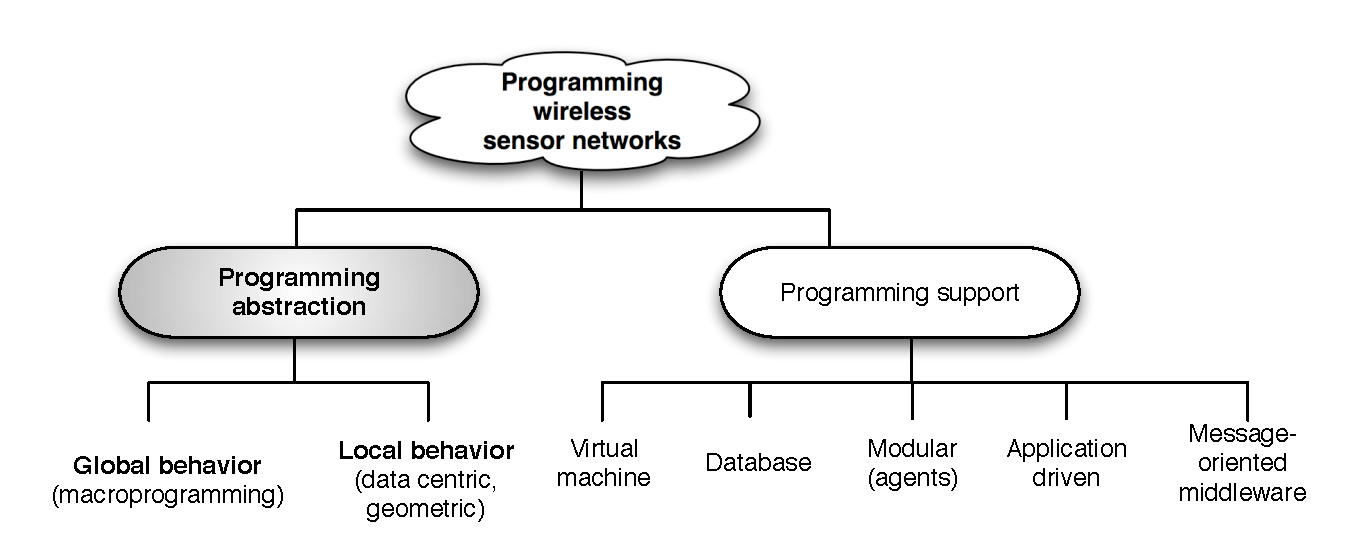
\includegraphics[width=\textwidth]{img/ProgrammingAbstractions.eps} 
\caption[Taxonomy of WSN programming models]{Taxonomy of WSN programming models (reproduced from
\cite{hadim_middleware:2006})}
\label{Fig:ProgrammingModels}
\end{figure}

Existing programming models for WSNs cover different areas and can serve 
several different purposes. They can be classified into two main types, depending on 
the applications they are used for  \cite{hadim_middleware:2006} (see Figure
\ref{Fig:ProgrammingModels}):
\begin{itemize}
\item \emph{Programming support}, wherein services and mechanisms allowing for 
reliable code distribution, safe code execution, etc. are provided. Some
examples of programming models that take this approach include Mate
\cite{Levis_Mate:2002}, Cougar \cite{Bonnet_Cougar:2001}, SOS
\cite{Han_SOS:2005}, and Agilla \cite{Fok_Agilla:2005}.
\item \emph{Programming abstractions}, where models deal with the global view 
of the WSN application as a system, and represent it through the concepts and 
abstractions of sensor nodes and sensor data. Some
examples of programming models that take this approach include TinyOS
\cite{levis_tinyOS:2005}, Kairos \cite{gummadi_Kairos:2005}, and
EnviroTrack \cite{Abdelzaher_EnviroTrack:2004}.
\end{itemize}

The rest of this section focuses on a description of WSN programming
abstractions.

\subsection{Classification of WSN Programming Abstractions}

\begin{figure}
\centering
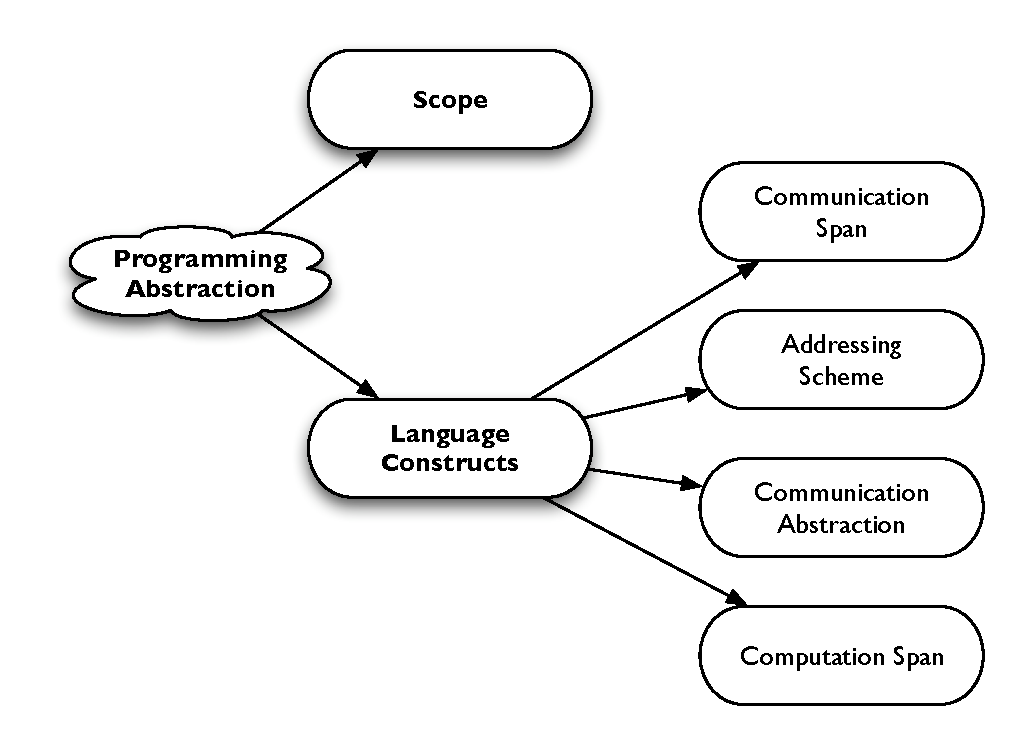
\includegraphics[scale=0.65]{img/ProgAbstr_Classification.eps}
\caption{Classification of Programming Abstractions} 
\label{Fig:ProgrAbstrClassification}
\end{figure} 

Programming abstractions may either be \emph{global} (also referred to 
as macroprogramming) or \emph{local} \cite{hadim_middleware:2006}. 

In the former case, the sensor network is programmed as a whole, and gets rid of
the notion of individual nodes \cite{mottola_middleware:2008}. Examples of
macroprogramming solutions include \emph{TinyDB} \cite{madden_TinyDB:2005} and
\emph{Kairos} \cite{gummadi_Kairos:2005}. 

In the latter case, the focus is on identifying relevant sections or
\emph{neighbourhoods} of the network. It is to be noted that these neighbourhoods
need not necessarily be physical. The framework used and developed during the
course of this work belongs to the latter class of programming abstractions.

Programming abstractions may also be classified on the basis of the
nature of the language constructs made available to the WSN programmer
\cite{mottola_middleware:2008}. Some of the metrics used for classification
are \cite{mottola_middleware:2008}:

\begin{itemize}
  \item \emph{Communication span}
  \item \emph{Addressing scheme}
  \item \emph{Communication abstraction}
  \item \emph{Computation span}
\end{itemize}

The rest of this section discusses each of these bases for classification in
detail, and is based on the work described in \cite{mottola_middleware:2008}
unless explicitly mentioned otherwise.

\subsubsection{Communication span}

The \emph{Communication span} enabled by a WSN programming interface is defined
as the set of nodes that communicate with one another in order to accomplish a
task. The communication span provided by a given abstraction can be:
\begin{itemize}
  \item \emph{Physical neighbourhood}
  \item \emph{Multi-hop group}
  \item \emph{System-wide}
\end{itemize}

Abstractions that use \emph{physical neighbourhood} approach provide
  the programmer with constructs to allow nodes to exchange data with others
  within direct communication range.
  
Abstractions with \emph{multi-hop group} approach allow the
  programmer to exchange data among subsets of nodes in the WSN using
  multi-hop communication. These sets may either be
  \emph{connected}, wherein there always exists a path between any two nodes in
  the set, or \emph{non-connected/disconnected}, where no such path
  exists.

\emph{System-wide} abstractions let the
  programmer use constructs that allow data exchange between any two nodes
  of the entire WSN. This may be seen as an extreme manifestation of the
  \emph{multi-hop group} approach mentioned above.

\subsubsection{Addressing scheme}

The \emph{addressing scheme} specifies the mechanism by which nodes are
identified. Typically, there are two kinds of addressing schemes used:

\begin{itemize}
  \item \emph{Physical addressing}
  \item \emph{Logical addressing}
\end{itemize}

In \emph{physical addressing} schemes nodes are identified using unique 
  identifiers. The same address always identifies the same node (or nodes, if
  duplicate  identifiers exist) at any time during the execution of the
  application.

When a \emph{logical addressing} mechanism is used, nodes are identified on the
basis of application-level properties specified by the application
programmer. Therefore, the same address, i.e. set of
application-level predicates, can identify different sets of nodes at different
times.

\subsubsection{Communication Abstraction}

This classification basis defines the degree to which details of communication
in a WSN are hidden from the application programmer's view. Programming
interfaces may provide either:

\begin{itemize}
  \item \emph{Explicit communication} primitives where the
  programmer working in the application layer has to handle communication
  aspects such as buffering and parsing.
  \item \emph{Implicit communication}, where the programmer is unaware of the
  details of the communication process, and communicates using
  high-level constructs.
\end{itemize}

\subsubsection{Computation Span}

The \emph{Computation span} enabled by a WSN programming interface is defined
as the set of nodes that can be affected by the execution of a single
instruction. The
computation span provided by a given abstraction can be:

\begin{itemize}
  \item \emph{Node}, when the effect of any instruction is restricted to a
  single node.
  \item \emph{Group}, where the programmer is provided with constructs that
  could affect a subset of nodes. 
  \item \emph{Global} present an extreme case of previous type, a single
  instruction can impact every node in the WSN.
\end{itemize}

 An example of this is WSN programming abstraction
 that allows the transmission of a message to all nodes in a WSN requiring the performance of a node reset if
 its sensor readings exceed a specific theshold.

\subsection{Programming models on the WSN protocol stack}

\begin{figure}
\centering
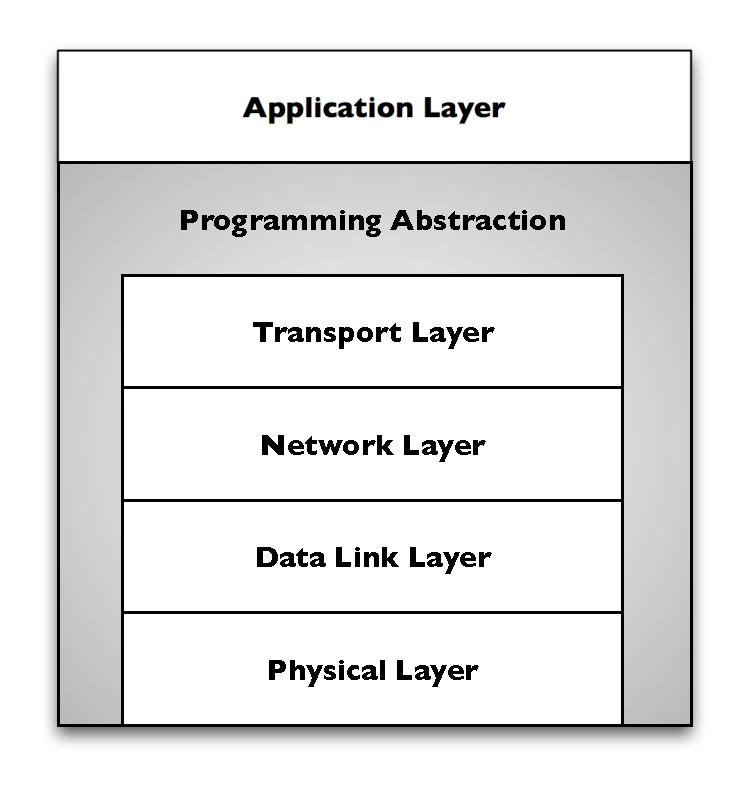
\includegraphics[scale=0.61]{img/ProtStack_ProgAbstr.eps}
\caption[Programming models on the WSN protocol stack]{Programming models on the WSN protocol
stack (adapted from \cite{mottola_middleware:2008})}
\label{Fig:ProtStack_ProgAbstr}
\end{figure}

WSN programming models are placed between the application layer and the
transport layer in the
protocol stack shown in Section \ref{sec:WSNProtStack}. As it can be seen from
Figure \ref{Fig:ProtStack_ProgAbstr},
fine-grained details are hidden from the application programmer's view. These
include:

\begin{itemize}
  \item Higher-layer services such as routing, localisation, and data storage
  mechanisms (and optimisations).
  \item Lower-layers such as the MAC protocol used, and the physical means of
  communication such as RF communication.
\end{itemize}

\section {Distributed Abstract Data Types} \label{sec:DADT}

Distributed Abstract Data Types are a new programming language construct used to
support distributed and context-aware applications. The concept of DADTs was
introduced in \cite{migliavacca_DADT:2006}. 
The rest of this section discusses the concepts and provides the reader with
the relevant background and examples\footnote{The examples provided are
adapted from \cite{migliavacca_DADT:2006}}.

\subsection{Abstract Data Types}

An Abstract Data Type (ADT) is the depiction of a model that
presents an abstract view to the problem at hand. This model of a problem
typically defines the affected data and the identified operations associated with
those.

The set of the data values and associated operations, independent of any
specific implementation, is called an ADT \cite{NIST_website}. From the
application developer's point of view, the use of ADTs allows for the separation of
interfaces from specific implementations.

One may consider a \emph{stack} a simple example of an ADT \cite{guttag_ADTs:1977}. It
can be represented through the stacked data, and a set of defined
operations that include \emph{push(data)}, \emph{pop()}, and \emph{top()}. It is intuitively clear that
several different implementations of an ADT may be defined using the proposed specification.

The concept of ADTs has been sucessfully used in several different areas of
science. The rest of this section focuses on the application and
extension of the concept of ADTs for use in WSNs.

\subsection{ADTs in WSNs} \label{subsubsec:ADTsinWSN}

A WSN as described earlier, usually consists of a number of sensor node. Each
sensor node may include several sensors.

\begin{figure}
\centering
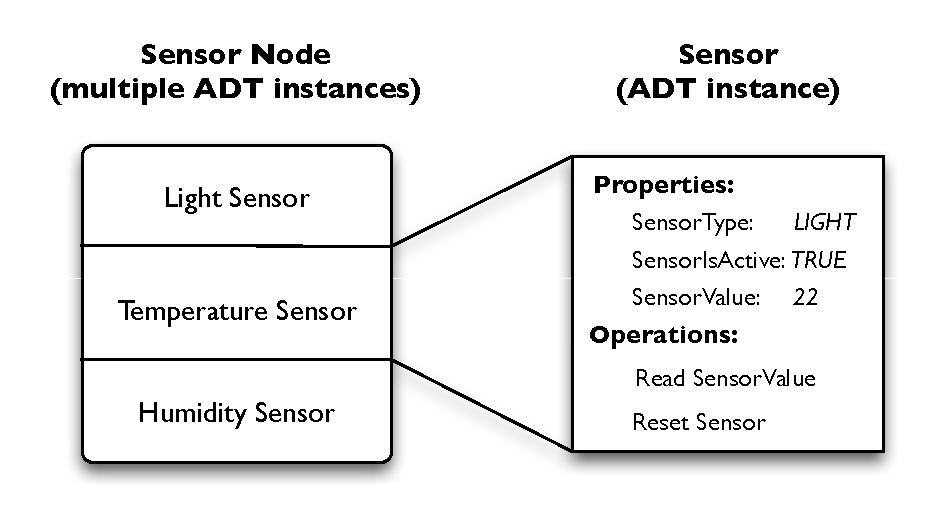
\includegraphics[scale=0.71]{img/ADTsMultipleInstances.eps}
\caption[Abstraction of sensor node through multiple ADTs]{Abstraction of sensor node through multiple ADTs}
\label{Fig:MultipleADTs}
\end{figure} 
  
Referring to the example in Figure \ref{Fig:MultipleADTs}, the ADT instance \emph{Sensor} can be used to abstract different types of sensors
that may be present on a sensor node. It specifies that a \emph{Sensor}
provides the list of common properties and operations. 
By declaration of multiple such ADT instances, the nature of the
wireless sensor node can be abstracted, as can be seen in the \emph{Sensor Node} entity shown in
Figure \ref{Fig:MultipleADTs}. This then allows the ADT instances to be used by the application
developer at a later point\footnote{Further details of ADT specification and
intantiation are provided in Section \ref{subsec:ADTSpecInst}}.

\subsection{Data and space ADTs} \label{subsubsec:DataAndSpaceADTs}

It is important to distinguish between data required by an application, and
the location, or space, where these providers of data reside. ADTs in WSNs can
provide not only the data from the sensor node, but also express a notion
of the ``computational environment'' hosting the data ADT.

Thus, ADTs be of two types:

\begin{itemize}
  \item \emph{Data ADTs}
  \item \emph{Space ADTs} 
\end{itemize}

\emph{Data ADTs} are ``conventional'' ADTs which encode application logic, such
as, for instance, allowing access to sensor data.

\emph{Space ADTs}, also known as \emph{sites}, are ADTs that provide an
abstraction of the computational environment (in the case of a WSN, a sensor
node) that ``hosts the data ADT'' \cite{migliavacca_DADT:2006}. The space ADT may
use different notions of space, such as physical location or network topology,
depending on application requirements as determined by the programmer.

\subsection{DADTs as an extension of ADTs} \label{subsec:DADTsConcepts}
Distributed ADTs (DADTs) are an extension of ADTs that make the state of multiple ADTs in a
distributed system collectively available.
\cite{migliavacca_DADT:2006}. 

\begin{figure}[h]
\centering
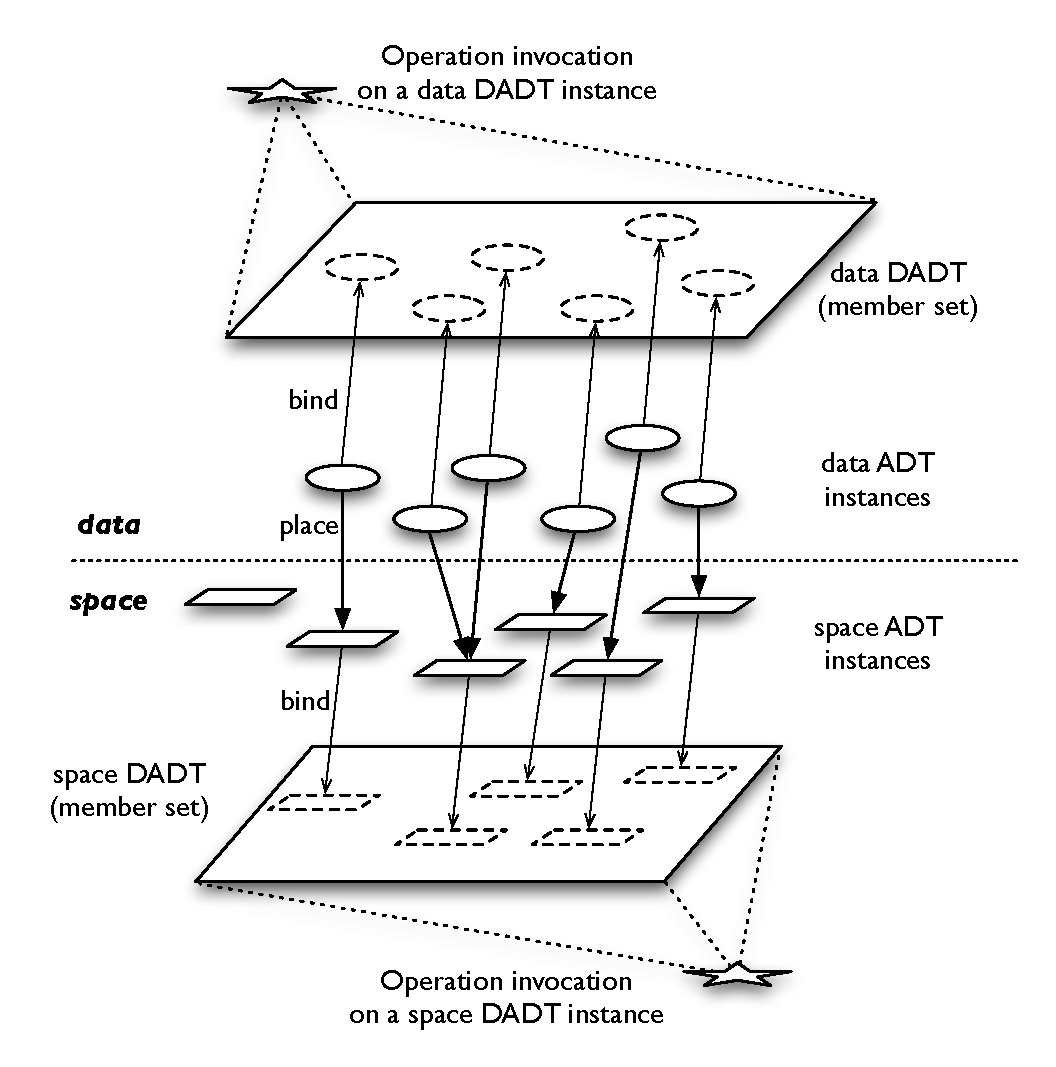
\includegraphics[scale=0.65]{img/DADTs.eps} 
\caption[Data and space in the DADT model]{Data and space in the DADT model (reproduced from 
\cite{migliavacca_DADT:2006})}
\label{Fig:DADTs}
\end{figure}

Similar to ADTs, DADTs 
provide specifications for distributed data, distributed operators, and 
constraints. The notion of space is extended to DADTs, and therefore DADTs can
either be (as it is shown in the Figure \ref{Fig:DADTs}):

\begin{itemize}
  \item \emph{Data DADT} that provide distributed access to a collection of data
  ADTs.
  \item \emph{Space DADT} that allows distributed access to a collection of
  space ADTs. 
\end{itemize}

The set of ADTs that are available for collective access using a DADT is called the \emph{member set} of
the DADT.

\subsubsection{DADT Operators and Actions} \label{subsubsec:OperatorsAndActions}

Operators are used in DADTs to declare distributed references to
the ADTs in the DADT member set. This reference conceals identities of individual ADT
instances from the application programmer. 

DADT operators may belong to one of the following types:

\begin{itemize}
  \item \emph{Selection Operators} that allow the performance of
  distributed operations on a subset of the instances in the member set.
  \item \emph{Conditional Operators} that provide support for global
  conditions to be applied on the member set prior to the execution of the DADT operation.
  \item \emph{Iteration Operators} that allow iterating over the
  ADT instances in the set, and thus permit access to individual ADT instances.
\end{itemize}

DADT actions are special DADT programming constructs. They are declared in the
DADT type, but are executed as an operation on remote ADT instances. 


\subsubsection{Views} \label{subsubsec:views}

\emph{DADT Views} permit the definition of the scope of distributed operations
that the application requires to perform. This approach is particularly useful
when a distributed operation has to be executed only on a subset of the
member set of ADT instances. The concept of DADT Views is presented in Figure
\ref{Fig:DADT_Views}.

\begin{figure}[h]
\centering
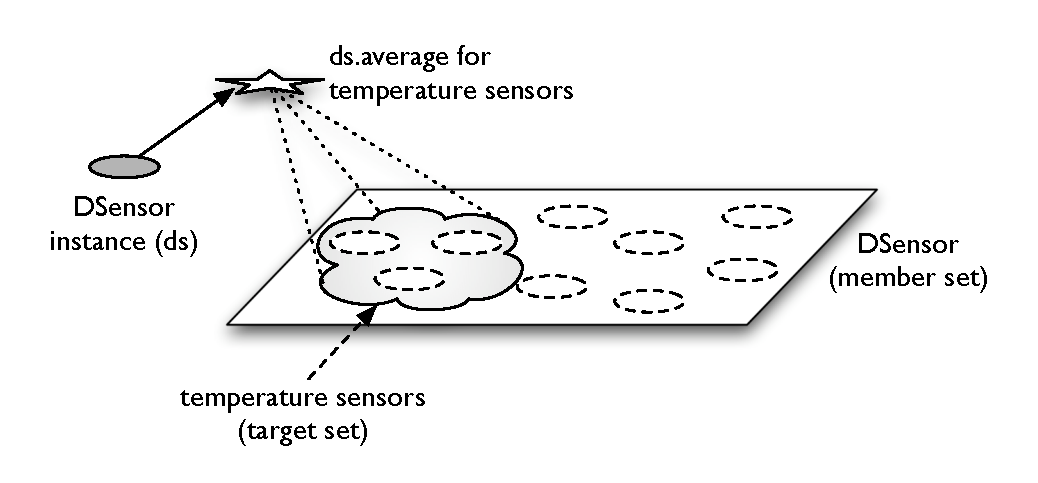
\includegraphics[scale=0.75]{img/DADT_Views.eps} 
\caption[DADT Views]{DADT views (reproduced from \cite{migliavacca_DADT:2006})}
\label{Fig:DADT_Views}
\end{figure}

The member set may be partitioned into DADT Views by using properties. A
\emph{Property} is a DADT characteristic that is defined in terms of an ADT's
data and operations, and is executed locally on the ADT instance
\cite{migliavacca_DADT:2006}.
DADT View may either be:
\begin{itemize}
  \item \emph{Data View},
  \item \emph{Space View}.
\end{itemize}


\section {Logical neighbourhoods} \label{LNDescription}

Typically, communication between WSN nodes is based on routing 
information between nodes by exploiting the communication radius of each node.
The notion of a node's physical neighbourhood - the set of nodes in the
network that fall within the communication range of a given node - is central to a mechanism of this nature.

However, in heterogenous WSN applications, the developer might require to
communicate with a specific subset of the network that is defined logically and
not physically. As an example of this, consider the following case. An
application that provides security in a high-risk environment by monitoring 
motion might require - in the event of a security alarm - all sensors at the
entrances to the guarded area to report about detected motion.
The sensors at the entrance form a logical neighbourhood in this case. However,
as the entrances may be widely separated, it is not necessary that these nodes
constitute part of a single physical neighbourhood.

The use of current WSN programming techniques to enable a mechanism of this
nature entails additional programming effort, because the developer has to deal
not only with the application logic, but also with the underlying problems of
transmitting messages to a specific logical neighbouhood while using lower layer
constructs that have no notion of this. This leads to increased code complexity
\cite{mottola_LN:2006}.

\begin{figure} 
\centering
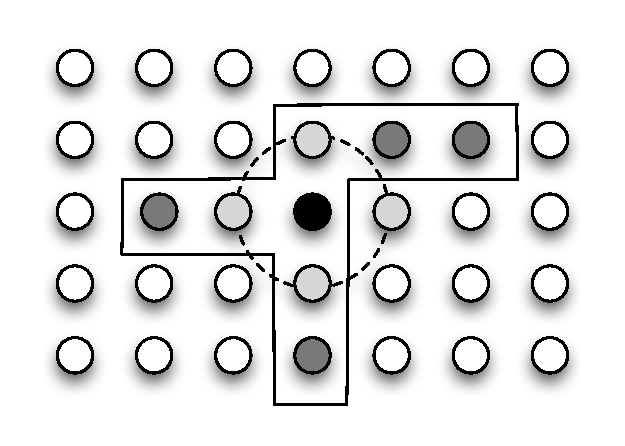
\includegraphics[scale=0.71]{img/LN_physical_vs_logical.eps} 
\caption[Difference between physical and logical neighborhoods]{Representation 
of logical and physical neighborhood of a given node. \emph{The dashed circle 
represents the physical neighborhood, whereas the solid polygon represents (one 
of the nodes in) the node's logical neighborhood} (reproduced from
\cite{mottola_LN:2006})}
\label{Fig:LN_physical_vs_logical}
\end{figure} 

Mottola and Picco \cite{mottola_LN:2006} suggest the addressing of the
aforementioned issues using \emph{Logical Neighbourhoods (LNs)}, an
abstraction that replaces the node's physical neighbourhood with a logical notion of
proximity (See Figure \ref{Fig:LN_physical_vs_logical}). Using this abstraction, programmers
can communicate with members of a LN using a simple message passing API,
thereby allowing for logical broadcasts. The implementation of this API is
supported by means of a novel routing mechanism devised specifically to support
LN communication.


The rest of this section discusses the LN abstractions and provides further
details of the underlying routing mechanism.

\subsection{The LN Abstraction}

LNs can be specified using a declarative language such as SPIDEY
\cite{mottola_LN:2006, mottola_LNScoping:2006}\footnote{The LN implementation
used as part of this work does not use a declarative language for LN specification}, and
involves the definition and instantiation of the \emph{node} and the
\emph{neighbourhood}. 

Nodes are a logical representation of the subset of a sensor node's state and
characterstics, and are used for the specification of an LN. Nodes are defined
in a node template and are subsequently instantiated, as shown in Listing \ref{listing:LN1}
   
A neighbourhood can be defined by applying predicates on the attributes defined
in the node template. The neighbourhood is defined using a neighbourhood
template, and subsequently instantiated.
   
\begin{lstlisting}[frame=trbl, basewidth={0.55em, 0.6em}, captionpos=b, 
basicstyle=\ttfamily\footnotesize, breaklines, caption = Node Definition and Instantiation, label = listing:LN1]  
node template Sensor
  static Function
  static Type
  dynamic BatteryPower
  dynamic Reading

create node ts from Sensor
  Function as "Sensor"
  Type as "Temperature"
  Reading as getTempReading()
  BatteryPower as getBatteryPower()
\end{lstlisting}


Listing \ref{listing:LN2} shows the definition and
instantiation of a
neighbourhood - based on the node template defined in Listing \ref{listing:LN1}
- which selects all temperature sensors where the reading exceeds a threshold.
 
\begin{lstlisting}[frame=trbl, basewidth={0.55em, 0.6em}, captionpos=b, 
basicstyle=\ttfamily\footnotesize, breaklines, caption = Neighbourhood Definition and Instantiation, label = listing:LN2]  
neighbourhood template HighTempSensors(threshold)
  with Function = "Sensor" 
      and Type  = "Temperature" 
      and Reading > Threshold

create neighbourhood HigherTemperatureSensors
  from HighTempSensors(threshold:45)
\end{lstlisting}

LN communication is enabled using a simple API that overrides the
traditionally used broadcast facility and makes it dependent on the (logical)
neighbourhood the message is addressed to \cite{mottola_LN:2006}. The routing mechanism described in
the next section enables LN commmunication.

\subsection{LN Routing}

The routing approach used in LNs is structure-less, and uses a local search
mechanism based on a distributed state space built by the periodic update of
node profiles. The routing mechanism can be divided into two phases \cite{mottola_LNAbstraction}:

\subsection{Construction of a distributed state space}
Each node periodically transmits a \emph{profile advertisement} that contains
information on the attribute-value pairs defined in the node template. This
message causes an update in its physical neighbours' \emph{State Space
Descriptors (SSDs)} if (a) no entry exists for any given attribute-value pair
specified in the profile advertisement, or (b) the \emph{transmit cost} is lower
than the costs for any existing SSD entry for a particular attribute-value pair.
If any such change occurs, the profile advertisement is rebroadcast with an
updated cost.

Additionally, passive listening to profile advertisements for attribute-value
pairs with higher costs than what is entered in the SDD is used to construct
increasing paths.

\subsection{ Routing through Local Search}
When a message has to be sent to a particular LN, the sending node transmits the
message to any node in its SSD whose attribute-value pairs match the LN
predicates. The message is associated with a specific set of \emph{credits} from
which the cost to send to the node is deducted. This process continues until the
message is received at node(s) in the LN along the reverse of the path, called
a \emph{decreasing path}, which is determined during the first phase. 

However, to ensure that messages are received by every nodes that belongs to the
neighbourhood (and the algorithm is not trapped in local state-space minima),
\emph{exploring paths} are used at specific points during the message traversal
(at nodes which meet the neighbourhood predicates, and/or after a user-defined
number of hops). The credit reservation system described above is used in that
case, with the node dividing the reserved credits between following decreasing
paths, and exploring paths.

\section {Sun SPOTs} \label{sec:sunspots}

Sensor nodes, as mentioned in Section \ref{subsec:sensornodes}, are
characterised by limited resources, including memory. 

In order to overcome memory limitations, wireless sensor network applications
have traditionally been coded in non-managed languages like C and assembly
language \cite{simon_squawk:2006}.
 
Managed runtime languages like Java were not used for sensor network programming
because of the combination of the static memory footprint of the Java Virtual
Machine (JVM) and the dynamic memory footprint of the WSN application code.
 
On the other hand, it is widely accepted that development times are greatly reduced
upon the use of managed runtime languages such as Java
\cite{simon_squawk:2006}. Therefore, currently prevalent WSN programming practice
trades developer efficiency for memory efficiency. 

However, Simon et al \cite{simon_squawk:2006} state the benefits resulted from
using a managed runtime language for WSN programming as follows:

\begin{itemize}
  \item Simplification of the process of WSN programming, that would cause an
  increase in developer adoption rates and productivity.
  \item Opportunity to use standard development and debugging tools.
\end{itemize}

The use of the Java programming language in SunSPOTs makes it particularly
suitable as a platform for the DADT applications presented. This is because the
DADT programming abstraction is designed to reduce programmer workload, and the
use of a managed runtime language such as Java has been shown to further
improve developer efficiency.
 
\subsection{The Sun SPOT hardware platform }
Sun Microsystems has, on the basis of the arguments discussed in the previous
section, proposed and built a sensor device
called the Sun Small Programmable Object Technology (Sun SPOT) that uses a
on-board JVM to allow for WSN programming using Java.

The Sun SPOT (see Figure \ref{Fig:SunSpot}) uses an ARM-9 processor, has 512 KB of RAM
and 4 MB of flash memory, uses a 2.4GHz radio with an integrated antenna on the board. The radio
is a TI CC2420 and is IEEE 802.15.4 compliant.

\begin{figure} 
\centering
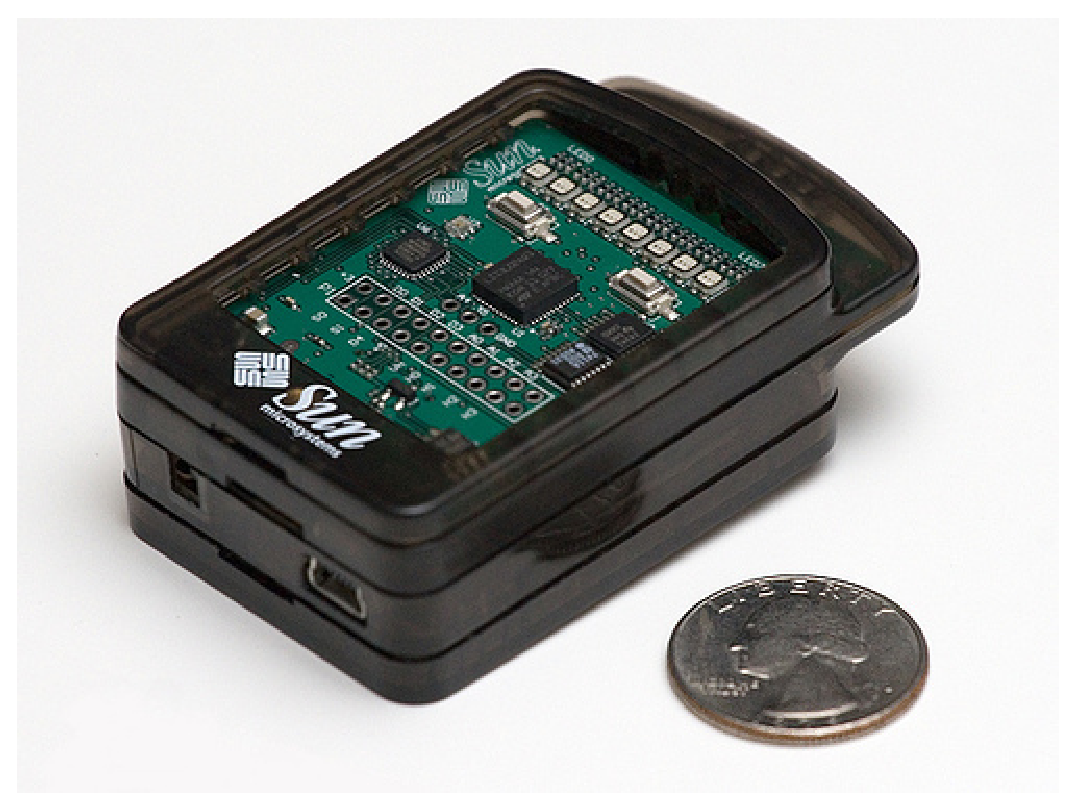
\includegraphics[scale=0.50]{img/sunspot1.eps} 
\caption[Sun SPOT device]{Sun SPOT device}
\label{Fig:SunSpot}
\end{figure} 


\subsection{The Squawk JVM}

The Squawk JVM is used on Sun SPOTs to enable on-board execution of Java
programs. The Squawk VM was originally developed for a smart card system with
even greater memory constraints than the Sun SPOTs. The Squawk JVM has the
following features \cite{simon_squawk:2006}:

\begin{itemize}
  \item It is written in Java, and specifically designed for resource
  constrained devices, meeting the requirements of Connected Limited Device
  Configuration 1.1 (CLDC) framework for Java Micro Edition (Java ME)
  applications.
  \item It does not require an underlying OS as it runs directly on the Sun
  SPOT hardware. This allows for a reduction in memory consumption.
  \item It suuports inter-device application migration.
  \item It allows the execution of multiple applications on one VM,
  representing each one as an object.
\end{itemize}

\subsection{Split VM Architecture}

As resource constrained devices are incapable of loading class files on-device
by virtue of their limited memory, a VM architecture known as the ``split VM
architecture'' is used, as shown in Figure
\ref{Fig:SquawkVM_architecture}.

\begin{figure}[h]
\centering
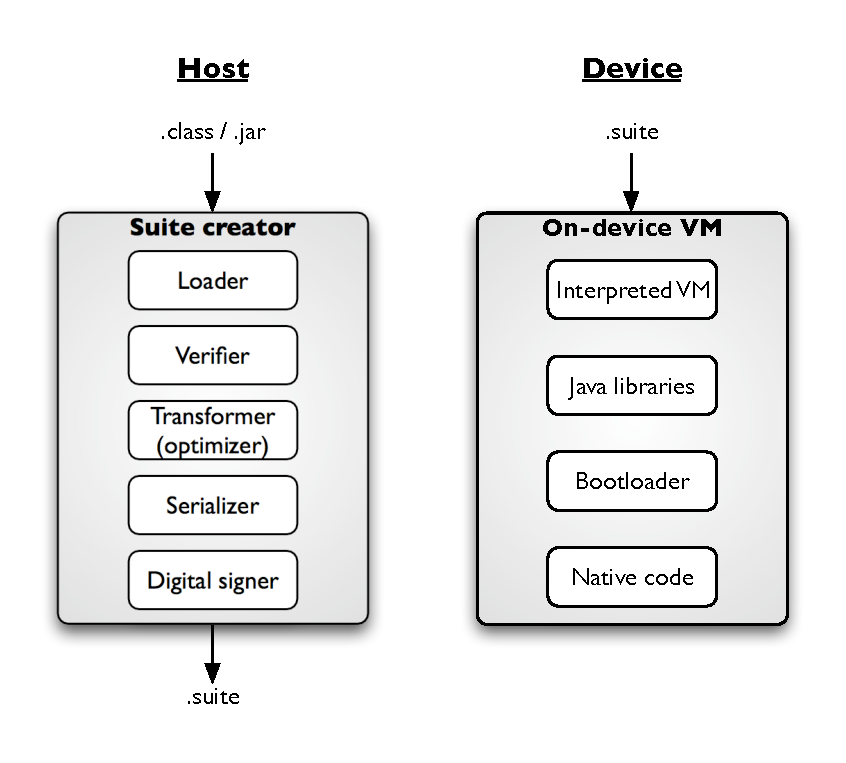
\includegraphics[scale=0.61]{img/Squawk_architecture.eps} 
\caption[The Squawk Split VM Architecture]{The Squawk
Split VM Architecture (reproduced from \cite{simon_squawk:2006})}
\label{Fig:SquawkVM_architecture}
\end{figure}  

The Squawk split VM architecture uses a class file preprocessor known as the
\emph{suite creator} that converts the \emph{.class} bytecode into a more
compact representation called the Squawk bytecode. According to
\cite{simon_squawk:2006}, Squawk bytecodes are optimised in order to:
\begin{itemize}
\item minimise space used by using smaller bytecode representation, escape
mechanisms for float and double instructions, and widened operands. 
\item enable in-place execution, by ``resolving symbolic references to other
classes, data members, and member functions into direct pointers, object offsets
and method table offsets respectively''.
\item simplify garbage collection, by the careful reallocation of local
variables, and by storing on the operand stack the operands of only those instructions that would result in a memory allocation.
\end{itemize}

The Squawk bytecodes are converted into a \emph{.suite} file created by
serialising and saving into a file the internal object memory representation.
These files are loaded on to the device, and subsequently interpreted by the
on-device VM.

\subsection{Sun SPOT applications} \label{subsec:sunspotapps}

Sun SPOT applications are divided into two classes:
\cite{sun_developer:2008}:

\begin{itemize}
  \item \emph{On-SPOT applications}
  \item \emph{On-Host applications}
\end{itemize}

\begin{figure}[h]
\centering
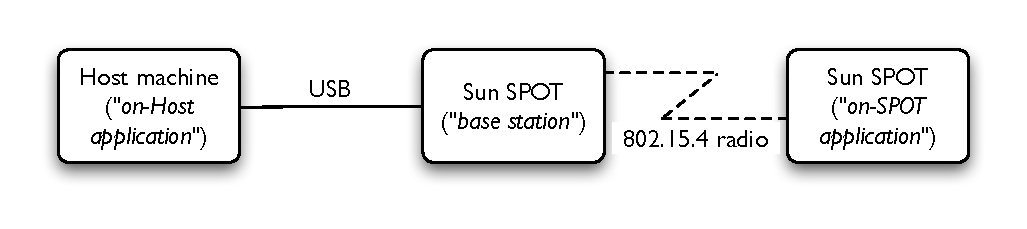
\includegraphics[width=\textwidth]{img/SunSPOTS_applications.eps} 
\caption[Types of Sun SPOT applications]{Types of Sun SPOT applications (adapted from
\cite{sun_developer:2008})}
\label{Fig:SunSPOTS_applications}
\end{figure}  

\emph{On-SPOT applications}  are deployed and
executed on a remote Sun SPOT that communicates untethered. On-SPOT
applications are Java programs that runs on the Squawk VM, and is compliant
with CLDC 1.1 specification. 

\emph{On-Host applications} run on the host machine
(typically a PC), and communicate with the network of Sun SPOTs through a base
station node that serves no purpose other than to facilitate Sun SPOT-host
machine communication. 
  
The base station node, which is a Sun SPOT itself, communicates with other
nodes in the network using RF communication, and with the host machine via a
USB link (see Figure \ref{Fig:SunSPOTS_applications}). The host application is
a Java 2 Standard Edition (J2SE) program.
  
 
\section{Summary}

This chapter presented an overview of the concepts, technologies, and hardware
underlying the work presented in this thesis. After underlining the need for the
use of programming models to increase the ubiquity of WSN use, this chapter
introduced a taxonomy of programming abstractions and placed the Distributed
Abstract Data Types programming abstraction used in this work within the
framework of the taxonomy. This was followed by a detailed discussion on Abstract
and Distributed Abstract Data Types used in the application layer of the
prototype produced during the course of this work, and the Logical Neighbourhood
routing mechanism used in the network and data link layers of the prototype. The
chapter concluded with a brief presentation of the SunSPOTs hardware platform,
and its particular suitability for the application under consideration. 


  